‌\section{Introducción}
Partiendo del diseño presentado en el trabajo anterior donde se buscó un sistema de venta de telefonía celular que permita tener un alto grado de confiabilidad tanto para el vendedor como para el cliente, que mantenga interconectadas a las distintas partes de la empresa (marketing - ventas - facturación - stock) en todo momento, que automatice algunos procesos internos de la empresa y que agilice y mejore el rendimiento de ventas, se presenta en este trabajo una segunda capa de modelos que pretende ilustrar la funcionalidad y comportamiento general del sistema.\\
\indent Como primer acercamiento a la utilización de la plataforma y su interacción con los distintos actores se incluyen una serie de Diagramas de Actividad en los que se despliegan tanto situaciones de uso abstractas y generales como también representaciones de casos puntuales tal y como se describiera en la sección \textsl{Escenarios} del primer informe. Luego se introduce un Modelo Conceptual con su especificación en $OCL$ con el objeto de \textbf{ME FALTA CHAMUYO ACÁ}. Como tercer acercamiento para entender la confección de este sistema se presentan diversos casos de uso con sus actores, modelo que está íntimamente relacionado con los primeros diagramas de actividad y que expande el detalle de estas interacciones.\\
\indent Por último, y no por eso menos importante, se incluye un modelo de Máquinas de Estados Finitos puesto que resultó oportuna su utilización para graficar de manera más formal cómo se comporta el sistema de ventas a la hora de tener que sincronizar procesos de la misma naturaleza que se realizan en paralelo y para los cuales es fundamental tener concurrencia con el stock de equipos de celular a modo de evitar falsas promesas y situaciones incómodas con los potenciales clientes.\\
\indent Es importante resaltar que a lo largo de este trabajo también se hace foco en la interconexión de estos modelos, característica denominada \textsl{trazabilidad}, la cual es fundamental para lograr comprender de manera integral el problema a través de los distintos documentos propuestos.\\

\section{Diagramas de Actividad}

En lo que respecta al comportamiento del sistema, puede decirse que existen tres flujos de actividad independientes: por un lado está la carga y descarga de stock, proceso que se lleva a cabo en el depósito correspondiente y que es fundamental para mantener un estado actualizado de las unidades en el sistema. Por otro lado se tiene la actividad del departamento de marketing, la cual -dejando de lado las distintas alternativas implementativas propuestas anteriormente- consiste lisa y llanamente en la alta y baja de promociones en el sistema. Finalmente, el tercer gran hilo de actividad paralela consiste en la visita de los distintos vendedores a clientes y la concreción de ventas. Mediante esta abstracción podemos sintetizar los fenómenos que interactúan en el sistema observando estas tres actividades y analizando cómo se relacionan entre sí.\\
\indent En la Figura~\ref{fig:da_ventaGral} se puede observar el DA correspondiente a una abstracción del proceso de venta mencionado. Resulta interesante notar que debido a la naturaleza de este modelo quedan implícitos los o-refinamientos correspondientes al diagrama de objetivos de la primera etapa del desarrollo de este sistema. Aquí se observa de manera transparente la interacción principal entre cliente y vendedor, y las acciones más importantes que realiza el vendedor sobre el sistema y éste de manera automática, ocultando las alternativas implementativas o comunicacionales. Esto pone el acento en el qué, y no en el cómo, dejando en claro el rol que juega cada actor de manera global. Otro aspecto que vale la pena destacar es que, más allá de la linealidad en el tiempo que presenta un circuito de flechas, el DA no permite representar fielmente un aspecto importante del sistema como lo es la ventana de tiempo de reserva de una promoción. Al pedir una reserva, el sistema realiza un chequeo de stock atómico mediante el cual, si hubiera disponibilidad, reserva las unidades para esa transacción durante 10 minutos. Durante este lapso el vendedor puede ultimar algunos detalles con el cliente y, principalmente, pedirle los datos a través de los cuales desea que se le facture la venta. Si bien esto se expresa en palabras, no se encontró una manera correcta dentro del modelo y que representara fielmente la situación en la cual se pudiera representar este lapso de tiempo durante el cual el cliente puede pedir la cancelación de la reserva (para cambiar de promoción o para simplemente no comprar nada) así como tampoco se pudo especificar que al agotarse el tiempo el sistema cancela la reserva automáticamente y se libera el stock restado. Este impedimento se verá subsanado en la sección \textbf{Máquinas de Estados Finitos} donde se modela el funcionamiento de los engranajes de la venta desde el sistema permitiendo enfatizar la sincronización y la temporalidad. Finalmente, ambos caminos terminan disparando en el sistema la finalización del workflow de venta.\\
\indent En cuanto al proceso de Stock, no resulta muy adecuado para especificar individualmente con este modelo puesto que no hay muchas interacciones y las pocas que hay resultan completamente asincrónicas, lo cual resulta muy difícil de comunicar correctamente en un DA. Por tal motivo se incluyó una parte de su funcionamiento en el DA de venta anterior, ya que en definitiva el envío al cliente de la mercadería forma parte del ciclo completo de una venta, sin embargo es importante recalcar que esto no necesariamente se produce inmediatamente después de la confirmación del departamento de Facturación, sino que el depósito de Stock tiene su propio esquema independiente de ingreso y egreso de mercadería. Por otro lado, también resulta oportuno recordar, según lo presentado en el anterior trabajo, que las unidades se quitan del stock del sistema al momento de la reserva y mientras esta no sea cancelada (ni su posterior facturación anulada), las unidades no se restituyen con lo cual el egreso de equipos es independiente de esta resta del sistema. Para las actividades restantes del área de stock se incluye el DA de la figura~\ref{fig:da_stock} en el que por decisión arbitraria la actividad descrita comienza mediante el envío de un pedido por parte de un proveedor. Es claro que este proceso es cíclico y fuera de fase, con lo cual no necesariamente el Encargado de Stock deberá primero recibir un pedido para realizar un encargo; nuevamente, esta es una de las limitaciones que provee el DA, no obstante tampoco amerita representarlo mediante FSM/LTS mientras que en este material presentado se logra una representación del flujo de acciones lo suficientemente inteligible.\\
\indent El tercer DA presentado en la figura~\ref{fig:da_marketing} corresponde a la especificación de uno de los métodos de creación de promociones por parte del departamento de Marketing. El mismo consiste en la creación de ofertas competitivas de manera automática: por un lado, los empleados de marketing cargan en el sistema distintos \textsl{datasources} los cuales quieren que sean monitoreados, y luego el sistema se encarga de recabar la información automáticamente y presentar un informe, que luego procesa por su cuenta para generar promociones automáticas. Notar que aquí, nuevamente, el DA presenta limitaciones en su poder de expresividad respecto al factor tiempo, ya que el grupo de marketing podría especificar distintas duraciones para cada configuración de monitoreo, desde horas, días, semanas, etc. Por otro lado, notar que si bien el sistema produce un conjunto de promociones, el énfasis está puesto en que el departamento revisa cada una individualmente, determinando si su confección es adecuada o si necesita ser manualmente corregida. Otra vez, el DA presenta cierta limitación a la hora de poder representar una serie de iteraciones o ciclos, puesto que a simple vista se entiende que se procesa una sola promoción, salvo por el hecho de la palabra ``cada'' en la leyenda de ese paso.\\

\begin{figure}[h!]
  \centering
  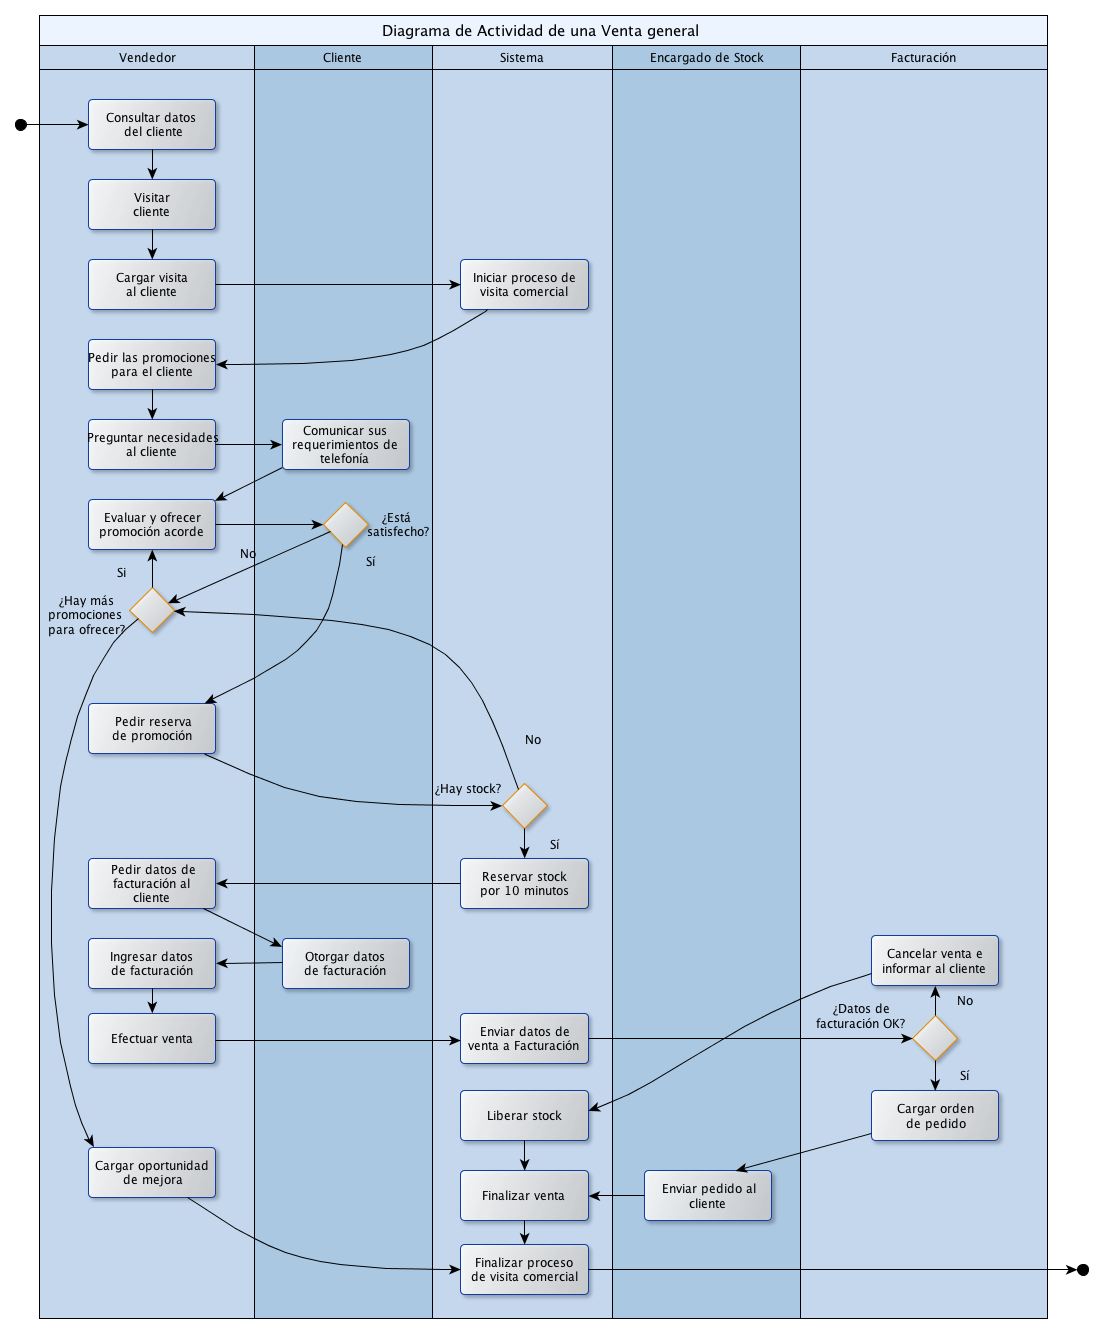
\includegraphics[width=1\textwidth]{./imagenes/da_general.png}
  \caption{DA de una venta general}
  \label{fig:da_ventaGral}
\end{figure}

\clearpage

\begin{figure}[h!]
  \centering
  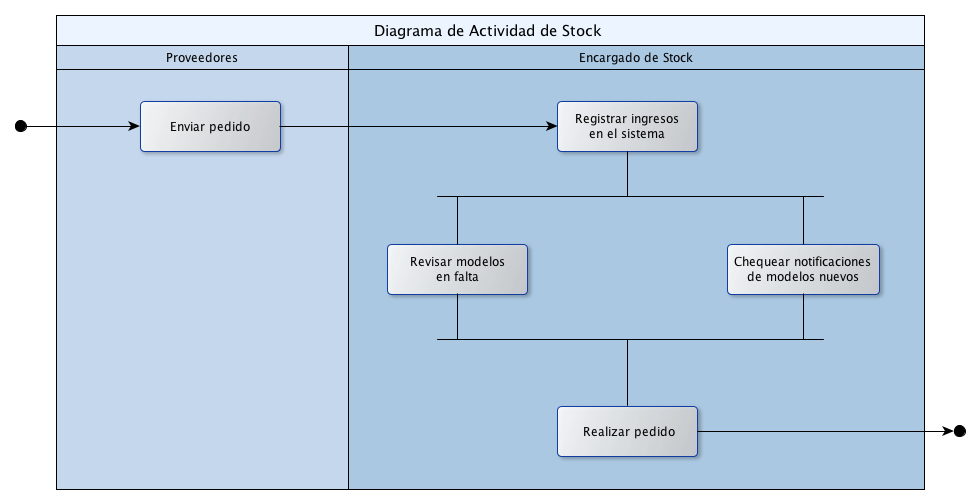
\includegraphics[width=1\textwidth]{./imagenes/da_stock.png}
  \caption{DA de un aspecto del proceso de control de Stock}
  \label{fig:da_stock}
\end{figure}

\begin{figure}[h!]
  \centering
  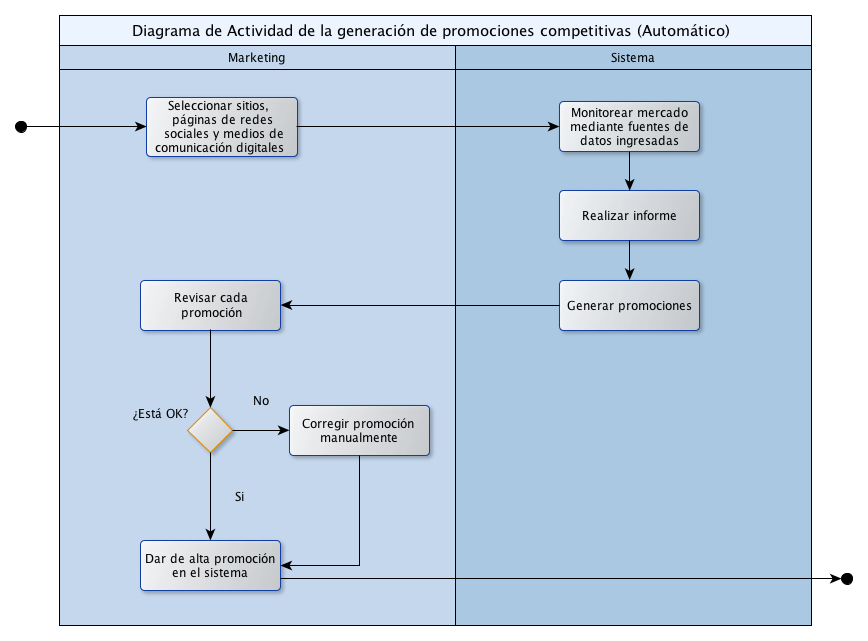
\includegraphics[width=1\textwidth]{./imagenes/da_marketing.png}
  \caption{DA de un aspecto de la creación de promociones por parte de Marketing}
  \label{fig:da_marketing}
\end{figure}

\clearpage

\section{Modelo Conceptual}

CHAMUYO!!

\begin{figure}[h!]
  \centering
  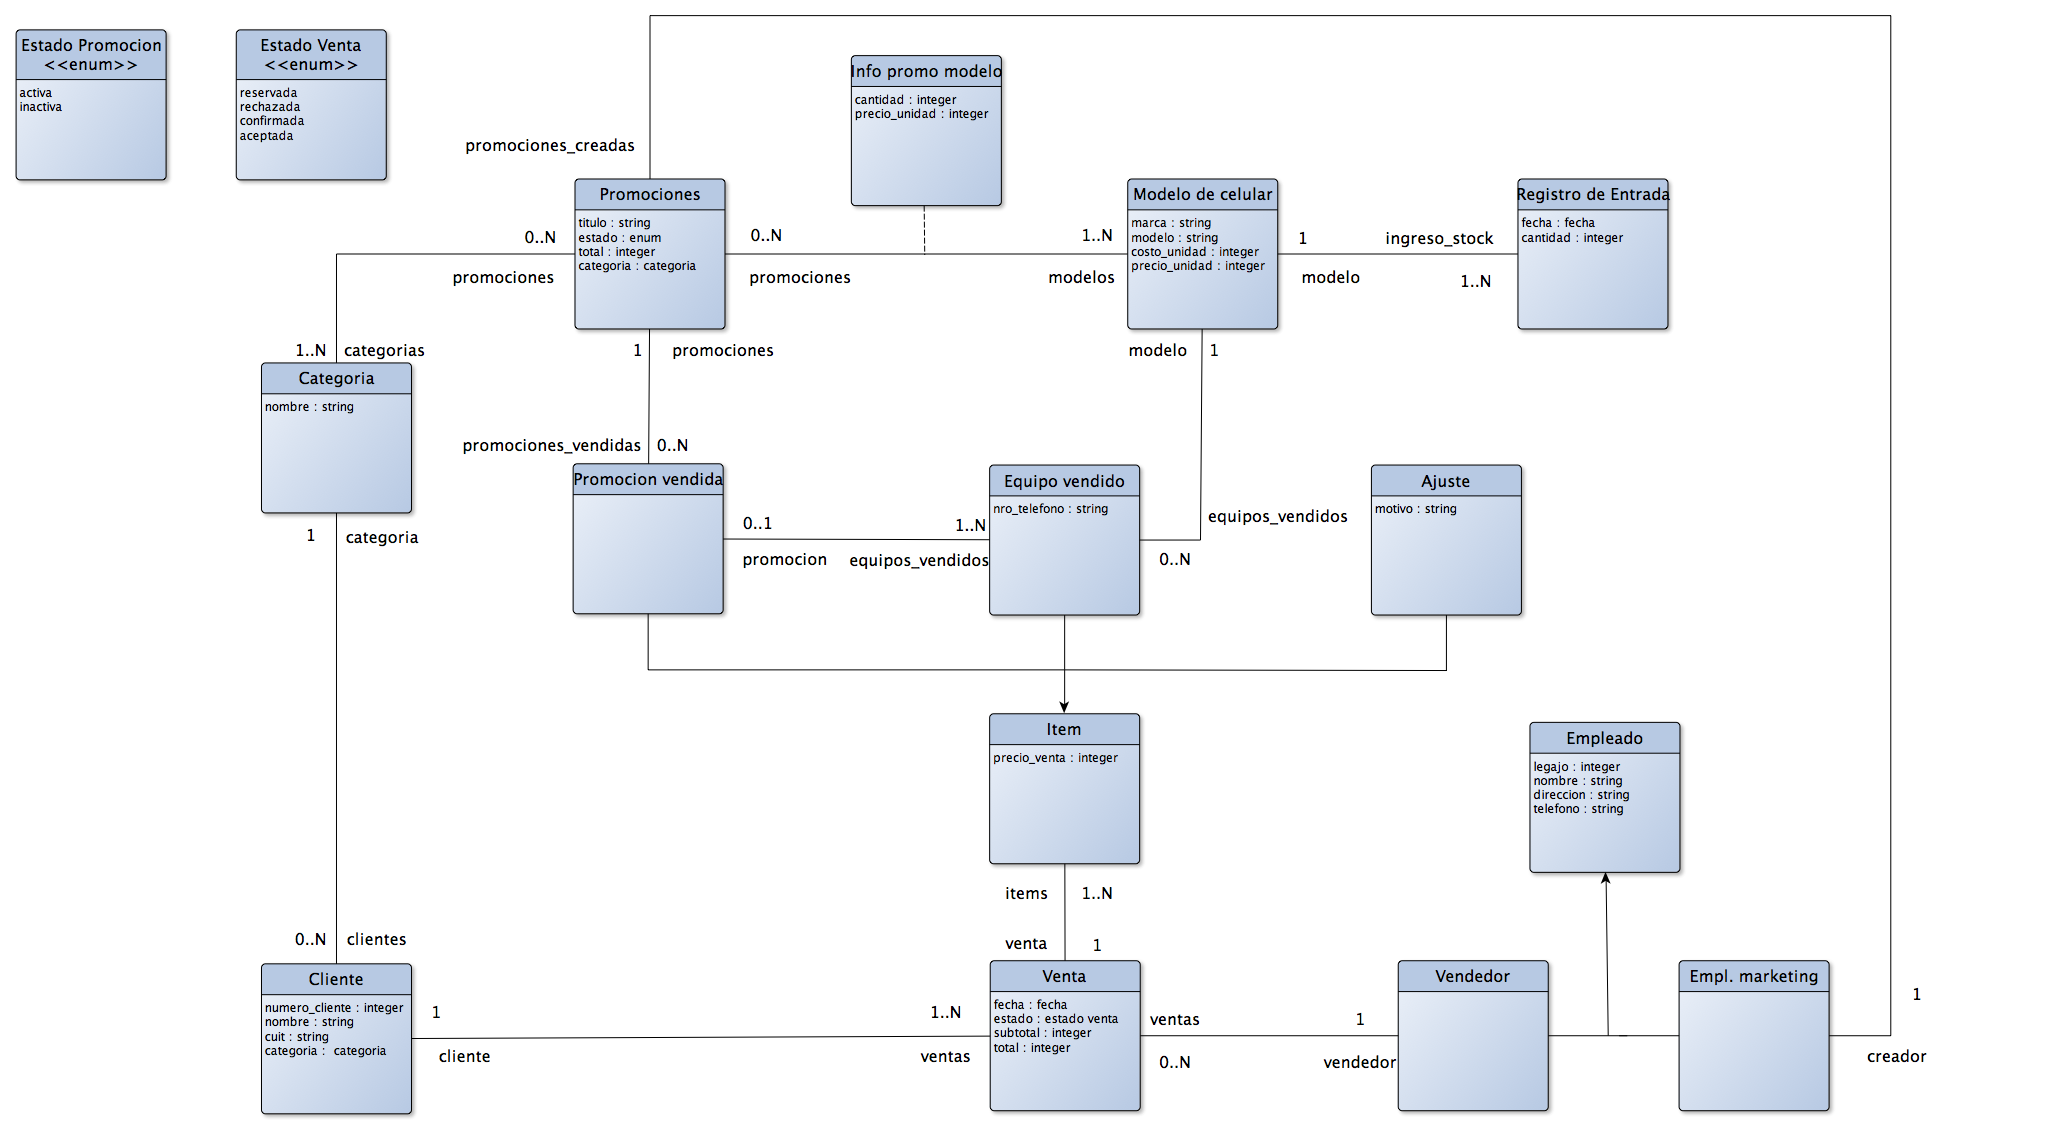
\includegraphics[width=1.5\textwidth, angle=90]{./imagenes/modelo_conceptual.png}
  \caption{Modelo conceptual}
  \label{fig:modelo_conceptual}
\end{figure}


\clearpage

\section{Casos de Uso}

\subsection{Casos de Uso MVP}

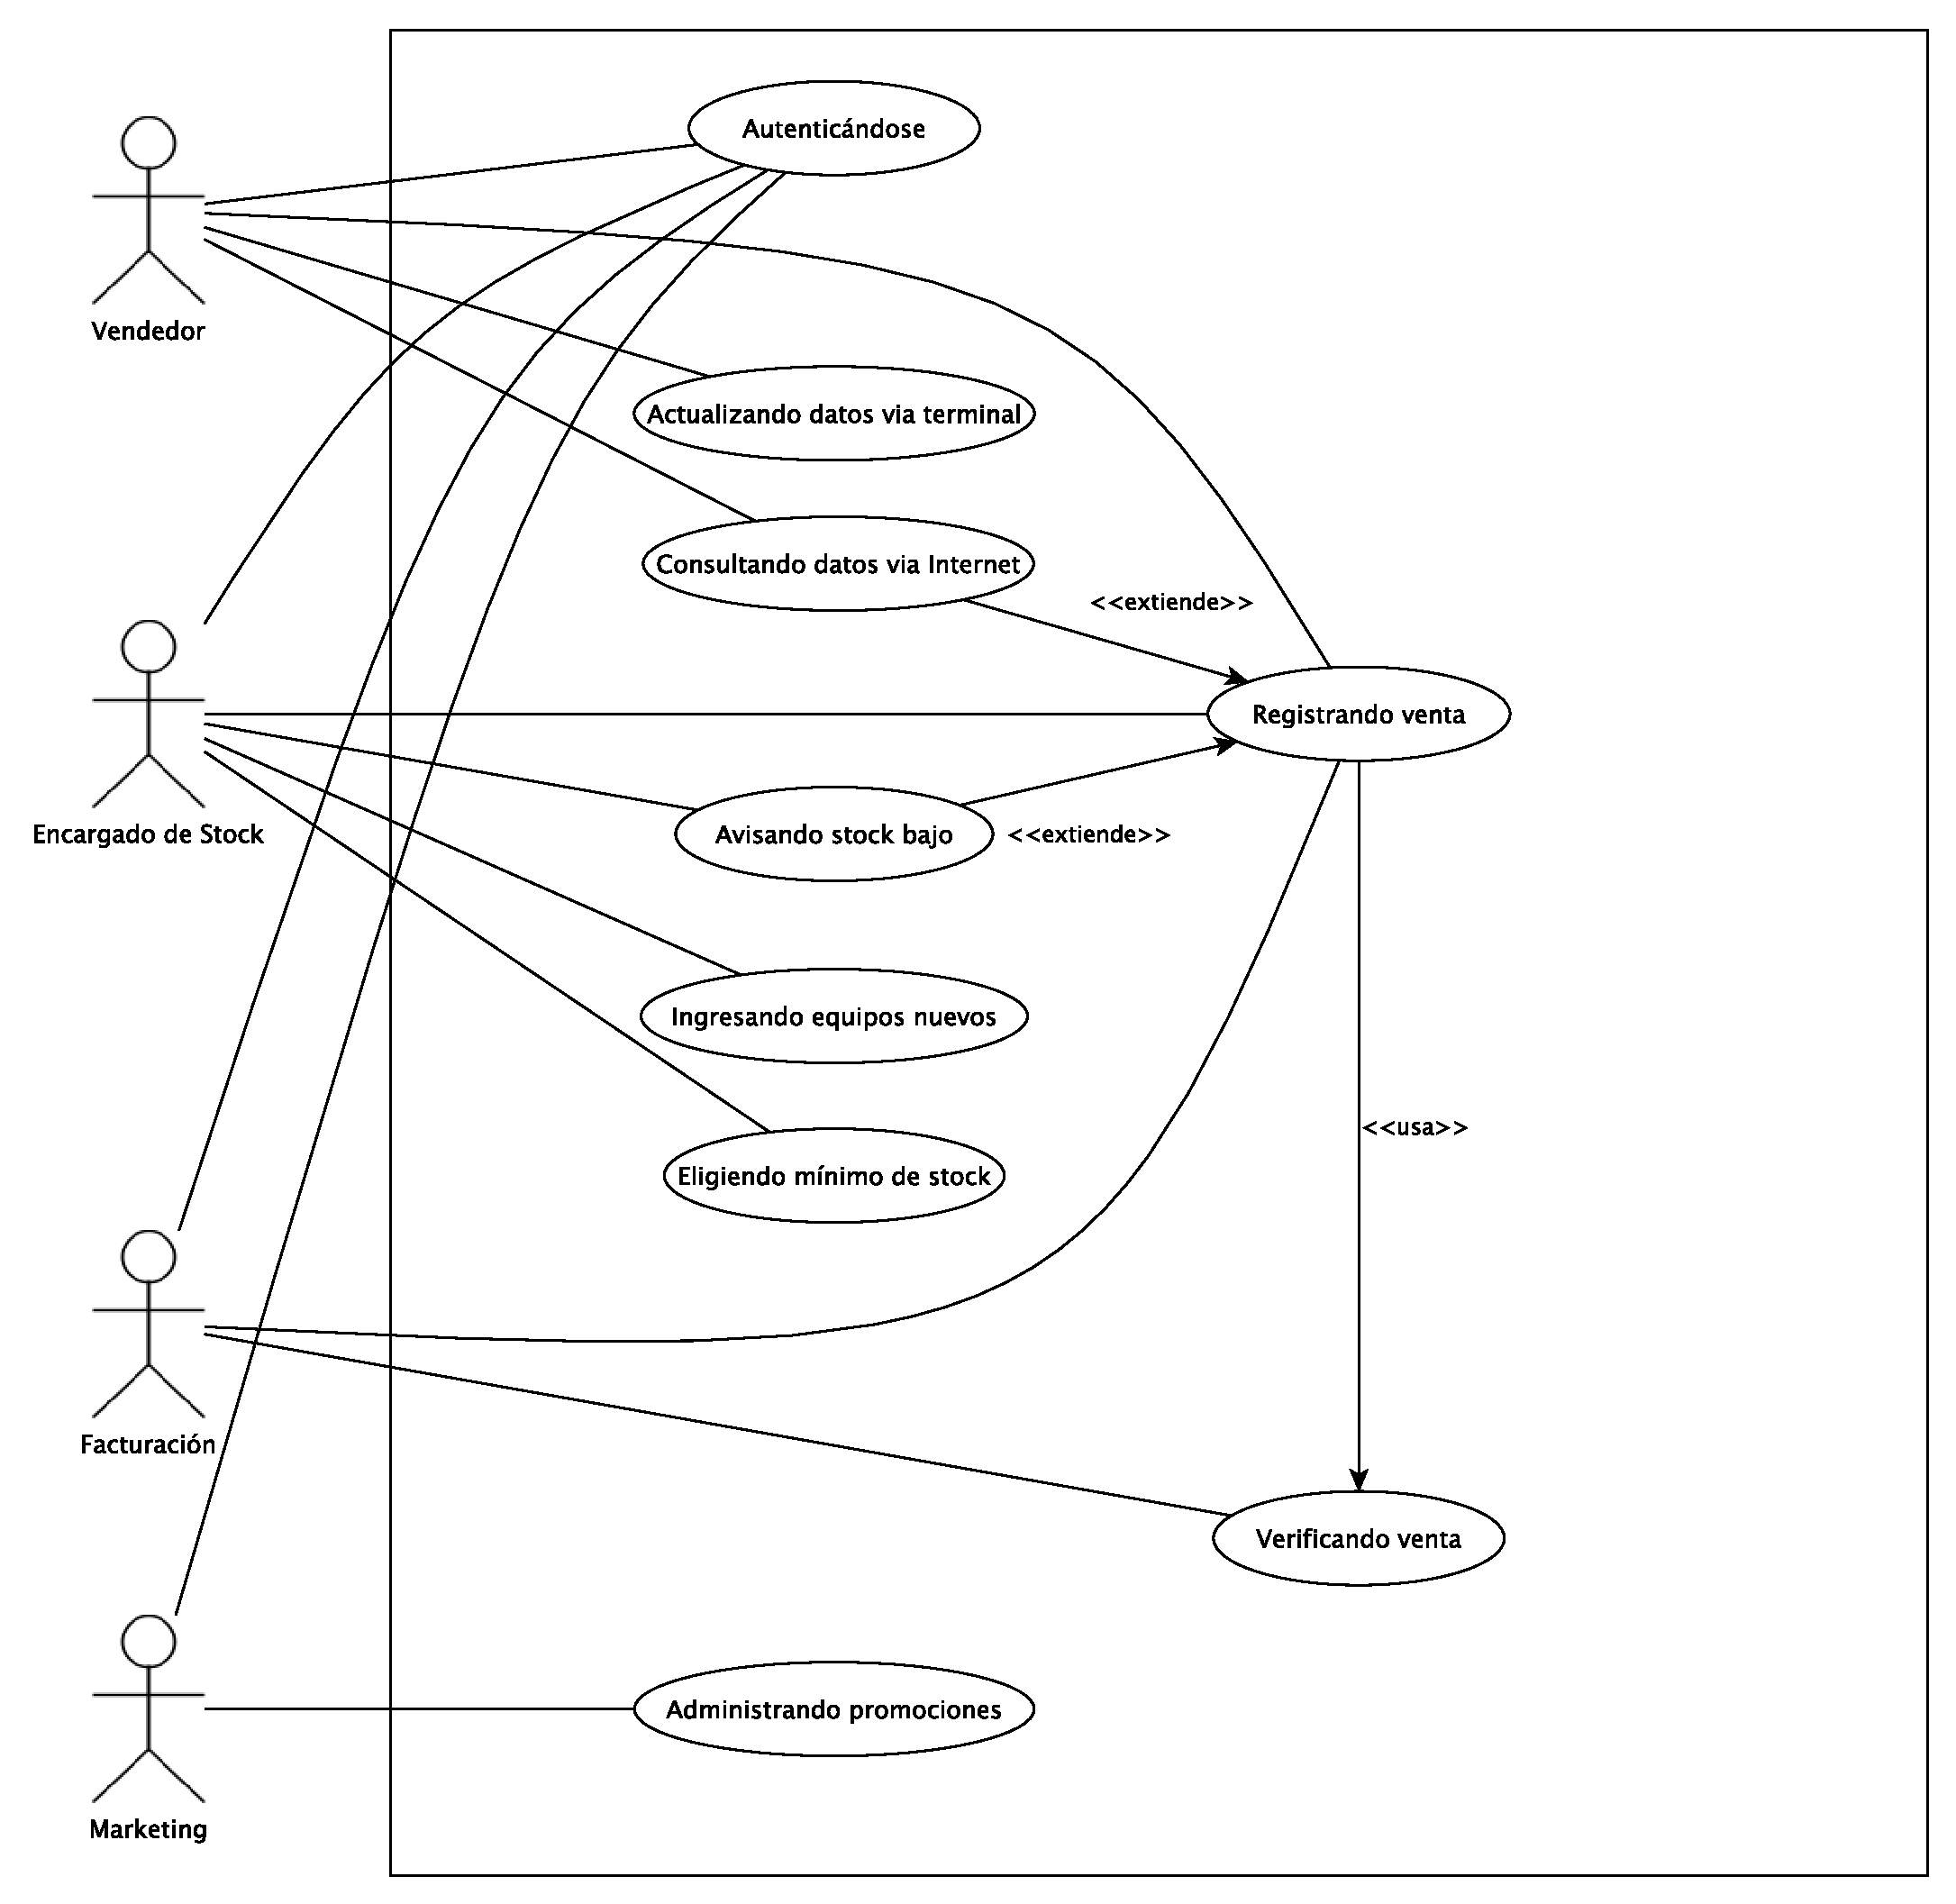
\includegraphics[width=1\textwidth]{./imagenes/casos_de_uso_mvp.pdf}

\subsubsection{Descripción de Casos de Uso}

\begin{tabular}{ | p{7cm} | p{7cm} | }
  \hline
  \multicolumn{2} {|l|} {Caso de Uso: Autenticándose.} \\
  \multicolumn{2} {|l|} {Actores: Vendedor, Encargado de Stock, Facturación, Marketing.} \\
  \multicolumn{2} {|l|} {Post: El usuario está autenticado en el sistema.} \\
  \hline
  Curso Normal & Curso Alternativo\\
  \hline
  1. El usuario ingresa a la interfaz web del sistema. & \\
  2. El usuario ingresa sus credenciales. & \\
  3. El sistema comprueba la validez de las credenciales y las acepta. & 3. El sistema comprueba la validez de las credenciales y las rechaza\\
  4. El usuario queda autenticado en el sistema. & 4. El usuario es redirigido al formulario para reingresar sus credenciales.\\
  \hline
\end{tabular}

\vspace{1cm}

\begin{tabular}{ | p{14cm} | }
  \hline
  Caso de Uso: Actualizando datos via terminal. \\
  Actores: Vendedor. \\
  Pre: El usuario está autenticado en el sistema. \\
  Post: El vendedor tiene actualizados en su dispositivo móvil promociones y datos de clientes. \\
  \hline
  Curso Normal\\
  \hline
  1. El vendedor enchufa su dispositivo móvil en una terminal del sistema ubicada en la oficina. \\
  2. El sistema actualiza automáticamente datos de promociones y clientes. \\
  \hline
\end{tabular}

\vspace{1cm}

\begin{tabular}{ | p{14cm} | }
  \hline
  Caso de Uso: Consultando datos via Internet. \\
  Actores: Vendedor. \\
  Pre: El usuario está autenticado en el sistema. \\
  Post: El vendedor recibe en su dispositivo móvil promociones y datos de clientes. \\
  \hline
  Curso Normal\\
  \hline
  1. El vendedor ingresa nombre del cliente que está visitando en su dispositivo móvil. \\
  2. El sistema busca los datos relacionados al cliente y promociones disponibles para él y los envía al dispositivo móvil del vendedor. \\
  \hline
\end{tabular}

\vspace{1cm}

\begin{tabular}{ | p{14cm} | }
  \hline
  Caso de Uso: Avisando stock bajo. \\
  Actores: Encargado de Stock. \\
  Pre: El usuario está autenticado en el sistema y el stock de alguno de los equipos asociado a promociones vigentes está pronto a agotarse. \\
  Post: El encargado de stock es notificado sobre el equipo pronto a agotarse. \\
  \hline
  Curso Normal\\
  \hline
  1. El sistema marca como reservados los equipos correspondientes con la promoción vendida.\\
  2. El sistema notifica al encargado de stock sobre los equipos reservados.\\
  \hline
\end{tabular}

\vspace{1cm}

\begin{tabular}{ | p{7cm} | p{7cm} | }
  \hline
  \multicolumn{2} {|l|} {Caso de Uso: Verificando venta.} \\
  \multicolumn{2} {|l|} {Actores: Facturación.} \\
  \multicolumn{2} {|l|} {Pre: El usuario está autenticado con el sistema y se registró una venta con stock disponible.} \\
  \multicolumn{2} {|l|} {Post: La venta se confirma y pasa al sistema de facturación.} \\
  \hline
  Curso Normal & Curso Alternativo\\
  \hline
  1. Facturación verifica la situación del cliente y aprueba la venta. & 1. Facturación verifica la situación del cliente y rechaza la venta. \\
  2. Se pasan los datos al sistema de facturación & 2. Se notifica al vendedor que la venta fue rechazada. \\
  \hline
\end{tabular}

\vspace{1cm}

\begin{tabular}{ | p{7cm} | p{7cm} | }
  \hline
   \multicolumn{2} {| p{10cm} |} {Caso de Uso: Registrando venta.} \\
   \multicolumn{2} {| p{10cm} |} {Actores: Vendedor, Encargado de Stock, Facturación.} \\
   \multicolumn{2} {| p{10cm} |} {Pre: El usuario está autenticado con el sistema y el vendedor tiene datos de clientes y promociones actualizados.} \\
   \multicolumn{2} {| p{10cm} |} {Post: Se registra una venta en el sistema.} \\
  \hline
  Curso Normal & Curso Alternativo\\
  \hline
  1. Se extiende con Consultando datos via Internet. & \\
  2. El vendedor decide junto al cliente qué promoción adquirir. & \\
  3. El vendedor ingresa elige en su dispositivo móvil la promoción que su cliente desea. & \\
  4. El sistema verifica que haya suficientes equipos en stock para satisfacer la promoción. & 4. El sistema verifica que los equipos en stock no alcanzan para satisfacer la promoción\\
  5. El sistema marca como reservados los equipos correspondientes con la promoción vendida. & 5. Se notifica al vendedor que la promoción no puede ser vendida. \\
  6. El sistema notifica al encargado de stock sobre los equipos reservados. & \\ 
  7. Se extiende con Avisando stock bajo. & \\
  8. Usa Verificando venta. & \\
  \hline
\end{tabular}

\vspace{1cm}

\begin{tabular}{ | p{14cm} | }
  \hline
  Caso de Uso: Ingresando equipos nuevos. \\
  Actores: Encargado de Stock. \\
  Pre: El usuario está autenticado con el sistema y nuevos equipos fueron ingresados al almacén. \\
  Post: Los nuevos equipos quedan dados de alta en el sistema. \\
  \hline
  Curso Normal\\
  \hline
  1. El usuario actualiza la cantidad de equipos correspondientes a los ingresados recientemente. \\
  \hline
\end{tabular}

\vspace{1cm}

\begin{tabular}{ | p{14cm} | }
  \hline
  Caso de Uso: Administrando promociones. \\
  Actores: Marketing. \\
  Pre: El usuario está autenticado con el sistema. \\
  Post: Se actualizan las promociones disponibles. \\
  \hline
  Curso Normal\\
  \hline
  1. El departamento de Marketing realiza un estudio de mercado para decidir qué promociones ofrecer según tipo de cliente. \\
  2. El usuario ingresado en el sistema crea, edita o borra una promoción. \\
  \hline
\end{tabular}

\subsection{Casos de Uso}

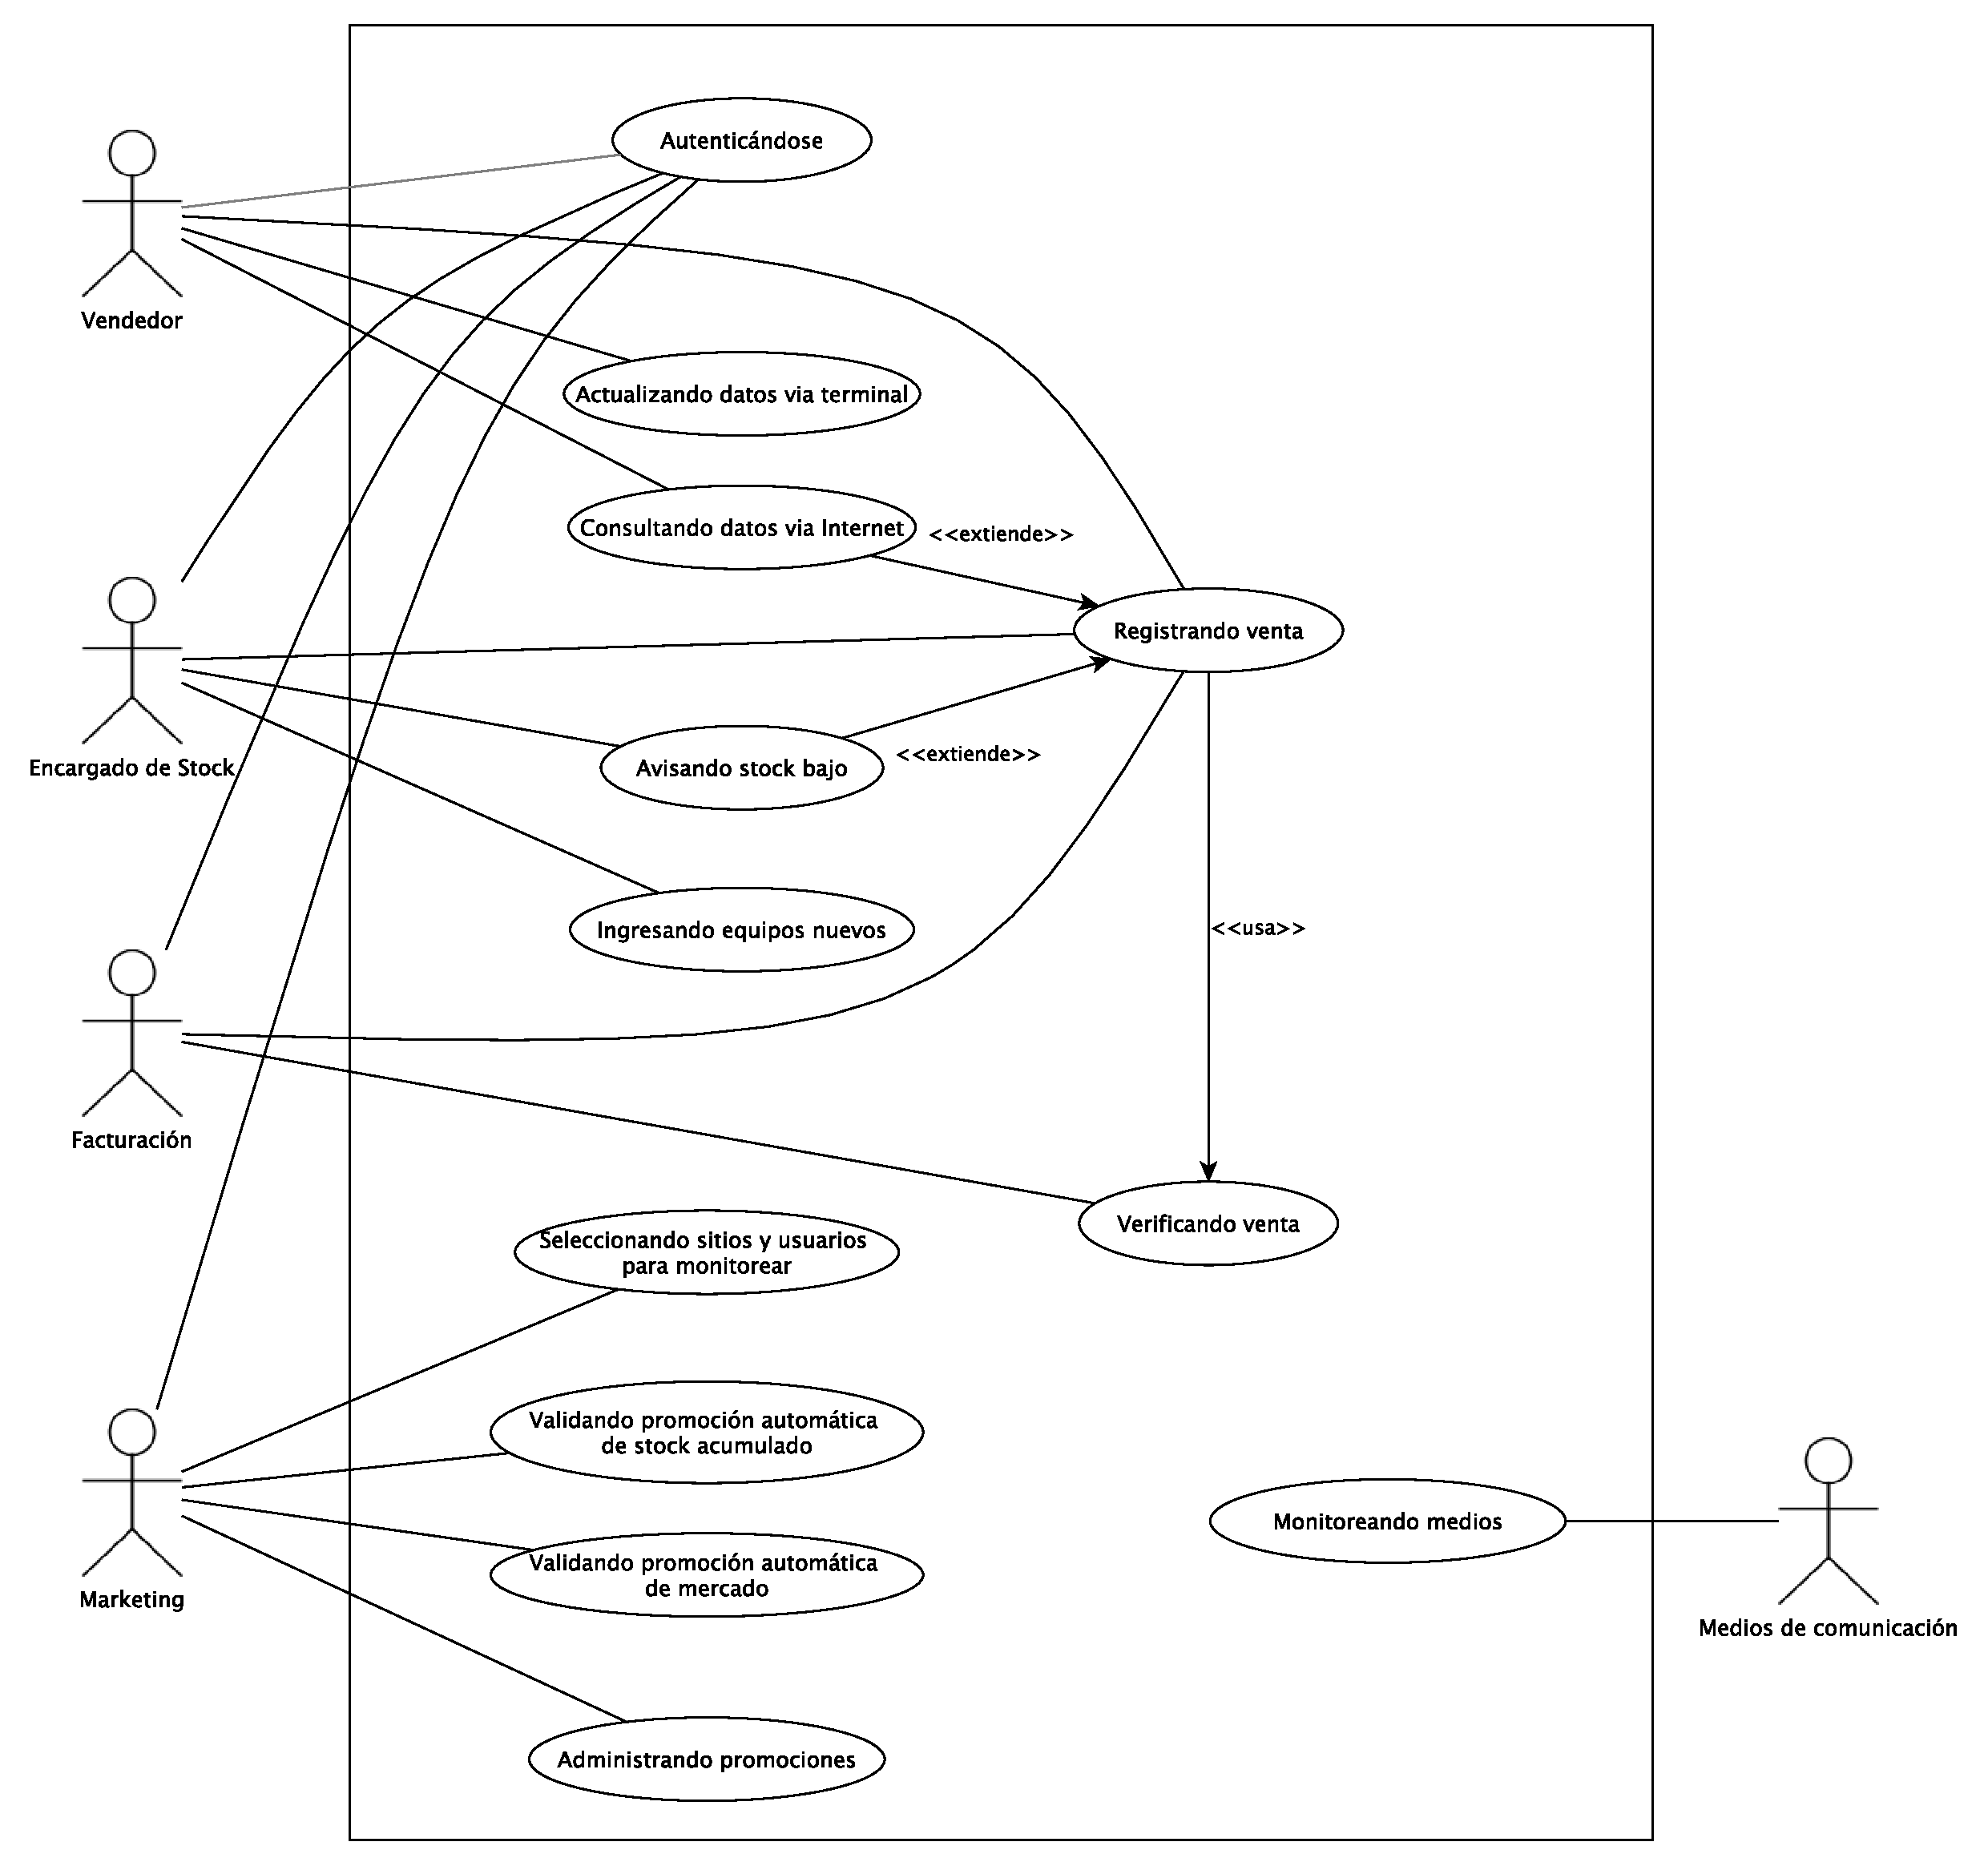
\includegraphics[width=1.1\textwidth]{./imagenes/casos_de_uso.pdf}

\clearpage

\subsubsection{Descripción de Casos de Uso}

\begin{tabular}{ | p{7cm} | p{7cm} | }
  \hline
  \multicolumn{2} {|l|} {Caso de Uso: Autenticándose.} \\
  \multicolumn{2} {|l|} {Actores: Vendedor, Encargado de Stock, Facturación, Marketing.} \\
  \multicolumn{2} {|l|} {Post: El usuario está autenticado en el sistema.} \\
  \hline
  Curso Normal & Curso Alternativo\\
  \hline
  1. El usuario ingresa a la interfaz web del sistema. & \\
  2. El usuario ingresa sus credenciales. & \\
  3. El sistema comprueba la validez de las credenciales y las acepta. & 3. El sistema comprueba la validez de las credenciales y las rechaza\\
  4. El usuario queda autenticado en el sistema. & 4. El usuario es redirigido al formulario para reingresar sus credenciales.\\
  \hline
\end{tabular}

\vspace{1cm}

\begin{tabular}{ | p{14cm} | }
  \hline
  Caso de Uso: Actualizando datos via terminal. \\
  Actores: Vendedor. \\
  Pre: El usuario está autenticado en el sistema. \\
  Post: El vendedor tiene actualizados en su dispositivo móvil promociones y datos de clientes. \\
  \hline
  Curso Normal\\
  \hline
  1. El vendedor enchufa su dispositivo móvil en una terminal del sistema ubicada en la oficina. \\
  2. El sistema actualiza automáticamente datos de promociones y clientes. \\
  \hline
\end{tabular}

\vspace{1cm}

\begin{tabular}{ | p{14cm} | }
  \hline
  Caso de Uso: Consultando datos via Internet. \\
  Actores: Vendedor. \\
  Pre: El usuario está autenticado en el sistema. \\
  Post: El vendedor recibe en su dispositivo móvil promociones y datos de clientes. \\
  \hline
  Curso Normal\\
  \hline
  1. El vendedor ingresa nombre del cliente que está visitando en su dispositivo móvil. \\
  2. El sistema busca los datos relacionados al cliente y promociones disponibles para él y los envía al dispositivo móvil del vendedor. \\
  \hline
\end{tabular}

\vspace{1cm}

\begin{tabular}{ | p{14cm} | }
  \hline
  Caso de Uso: Avisando stock bajo. \\
  Actores: Encargado de Stock. \\
  Pre: El usuario está autenticado en el sistema y l stock de alguno de los equipos asociado a promociones vigentes está pronto a agotarse. \\
  Post: El encargado de stock es notificado sobre el equipo pronto a agotarse. \\
  \hline
  Curso Normal\\
  \hline
  1. El sistema marca como reservados los equipos correspondientes con la promoción vendida.\\
  2. El sistema notifica al encargado de stock sobre los equipos reservados.\\
  \hline
\end{tabular}

\vspace{1cm}

\begin{tabular}{ | p{7cm} | p{7cm} | }
  \hline
  \multicolumn{2} {|l|} {Caso de Uso: Verificando venta.} \\
  \multicolumn{2} {|l|} {Actores: Facturación.} \\
  \multicolumn{2} {|l|} {Pre: El usuario está autenticado con el sistema y se registró una venta con stock disponible.} \\
  \multicolumn{2} {|l|} {Post: La venta se confirma y pasa al sistema de facturación.} \\
  \hline
  Curso Normal & Curso Alternativo\\
  \hline
  1. Facturación verifica la situación del cliente y aprueba la venta. & 1. Facturación verifica la situación del cliente y rechaza la venta. \\
  2. Se pasan los datos al sistema de facturación & 2. Se notifica al vendedor que la venta fue rechazada. \\
  \hline
\end{tabular}

\vspace{1cm}

\begin{tabular}{ | p{7cm} | p{7cm} | }
  \hline
   \multicolumn{2} {| p{10cm} |} {Caso de Uso: Registrando venta.} \\
   \multicolumn{2} {| p{10cm} |} {Actores: Vendedor, Encargado de Stock, Facturación.} \\
   \multicolumn{2} {| p{10cm} |} {Pre: El usuario está autenticado con el sistema y el vendedor tiene datos de clientes y promociones actualizados.} \\
   \multicolumn{2} {| p{10cm} |} {Post: Se registra una venta en el sistema.} \\
  \hline
  Curso Normal & Curso Alternativo\\
  \hline
  1. Se extiende con Consultando datos via Internet. & \\
  2. El vendedor decide junto al cliente qué promoción adquirir. & \\
  3. El vendedor ingresa elige en su dispositivo móvil la promoción que su cliente desea. & \\
  4. El sistema verifica que haya suficientes equipos en stock para satisfacer la promoción. & 4. El sistema verifica que los equipos en stock no alcanzan para satisfacer la promoción\\
  5. El sistema marca como reservados los equipos correspondientes con la promoción vendida. & 5. Se notifica al vendedor que la promoción no puede ser vendida. \\
  6. El sistema notifica al encargado de stock sobre los equipos reservados. & \\ 
  7. Se extiende con Avisando stock bajo. & \\
  8. Usa Verificando venta. & \\
  \hline
\end{tabular}

\vspace{1cm}

\begin{tabular}{ | p{14cm} | }
  \hline
  Caso de Uso: Ingresando equipos nuevos. \\
  Actores: Encargado de Stock. \\
  Pre: El usuario está autenticado con el sistema y nuevos equipos fueron ingresados al almacén. \\
  Post: Los nuevos equipos quedan dados de alta en el sistema. \\
  \hline
  Curso Normal\\
  \hline
  1. El usuario actualiza la cantidad de equipos correspondientes a los ingresados recientemente. \\
  \hline
\end{tabular}

\vspace{1cm}

\begin{tabular}{ | p{14cm} | }
  \hline
  Caso de Uso: Administrando promociones. \\
  Actores: Marketing. \\
  Pre: El usuario está autenticado con el sistema. \\
  Post: Se actualizan las promociones disponibles. \\
  \hline
  Curso Normal\\
  \hline
  1. El departamento de Marketing realiza un estudio de mercado para decidir qué promociones ofrecer según tipo de cliente. \\
  2. El usuario ingresado en el sistema crea, edita, borra, activa o desactiva una promoción. \\
  \hline
\end{tabular}

\vspace{1cm}

\begin{tabular}{ | p{14cm} | }
  \hline
  Caso de Uso: Seleccionando sitios y usuarios para monitorear. \\
  Actores: Marketing. \\
  Pre: El usuario está autenticado con el sistema. \\
  Post: El sistema puede comenzar a monitorear medios. \\
  \hline
  Curso Normal\\
  \hline
  1. El usuario selecciona qué usuarios de redes sociales y sitios corporativos el sistema deberá monitorear. \\
  \hline
\end{tabular}

\vspace{1cm}

\begin{tabular}{ | p{14cm} | }
  \hline
  Caso de Uso: Validando promoción automática de stock acumulado. \\
  Actores: Marketing. \\
  Pre: El usuario está autenticado con el sistema. \\
  Post: Se crea una promoción en base al stock acumulado, autorizada por Marketing. \\
  \hline
  Curso Normal\\
  \hline
  1. El sistema detecta que se acumuló mucho stock de un determinado equipo. \\
  2. El sistema crea una promoción basada en el stock acumulado de dicho equipo y notifica al usuario. \\
  3. El usuario ve la promoción, la modifica si considera necesario y la activa. \\
  4. La promoción pasa a estar disponible para los vendedores. \\
  \hline
\end{tabular}

\vspace{1cm}

\begin{tabular}{ | p{14cm} | }
  \hline
  Caso de Uso: Validando promoción automática de mercado. \\
  Actores: Marketing. \\
  Pre: El usuario está autenticado con el sistema y el sistema monitoreó los medios de comunicación. \\
  Post: Se crea una promoción en base al estado del mercado, autorizada por Marketing. \\
  \hline
  Curso Normal\\
  \hline
  1. El sistema envía un informe con los detalles del estado del mercado al usuario. \\
  2. El sistema fabrica una promoción en base al informe. \\
  3. El usuario ve la promoción, la modifica si considera necesario y la activa. \\
  4. La promoción pasa a estar disponible para los vendedores. \\
  \hline
\end{tabular}

\vspace{1cm}

\begin{tabular}{ | p{14cm} | }
  \hline
  Caso de Uso: Monitoreando medios.\\
  Actores: Medios de Comunicación. \\
  Pre: Se seleccionaron sitios y usuarios para monitorear. \\
  Post: El sistema realizó el monitoreo de los medios de comunicación en Internet según las preferencias seleccionadas. \\
  \hline
  Curso Normal\\
  \hline
  1. El sistema monitorea los medios de comunicación por internet asociados a los usuarios de redes sociales y sitios de la competencia. \\
  \hline
\end{tabular}
